
\hypertarget{menu_search}{}
\section{Search}
\index{search menu}

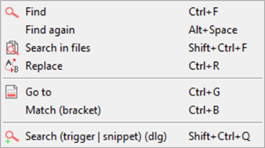
\includegraphics[scale=0.8]{./res/menu_search.png}\\

\begin{scriptsize}
  \begin{tabularx}{\textwidth}{>{\hsize=0.2\hsize}X>{\hsize=.8\hsize}X}\\
    \hline
    \textbf{Option} & \textbf{Description} \\
    \hline
    Find & Opens the \href{\#working\_find\_replace}{Find} dialog \\
    Find again & Uses the previously entered search criteria to find the next occurrence,
    i.e, one closer to the end of the file. This option is not available if a search has not been carried out. \\
    Search in files & Opens the \href{\#working\_search\_in\_files}{Search in files} dialog \\
    \hdashline[1pt/1pt]
    Replace & Opens the \href{\#working\_find\_replace}{Replace} dialog \\
    Go to & This option produces the dialog below and allows you to move the cursor to the specified position \\
    Match bracket & Search for matching bracket. See details below \\
    \hdashline[1pt/1pt]
    Search (trigger | snippet) (dlg) & Open window (dlg) for efficient search of triggers and snippets.
    \textit{\href{\#additional_dialogs_search_trigger}{See more details ...}} \\
    \hline
  \end{tabularx}
\end{scriptsize}

\begin{description}
  \item[How to match:]
    The cursor must be placed immediately before any of the bracket characters.
     When this option is called the cursor will move to the point immediately before the matching bracket.

  \item[Recognized brackets:]
    The bracket characters are (), [] and \{\}.
\end{description}
